
\section{Results}

\subsection{Scenario Filtering}

\begin{frame}
  \frametitle{Scenario filtering}
    Scenarios we filtered the dataset with:
    \begin{itemize}[<+->]
      \item Lane merging
      \item Lane exiting 
      \item Entering behaviour
      \item Exiting behaviour
    \end{itemize}
\end{frame}

\begin{frame}
    \center Video demo of the scenarios
\end{frame}


\subsection{Integration Method}

\begin{frame}
  \frametitle{Reminder: Our Model - Matrix Form}
    Acceleration from Distance formula:
    \begin{align*}
        \begin{bmatrix} a(k) \\ \end{bmatrix}
        &=
        \begin{bmatrix}
            -a(k-1)  & v(k+1) - v(k)   \\ 
        \end{bmatrix}
        \begin{bmatrix}
            \overline{\textcolor{red}{c_1}} \\
            \overline{\textcolor{red}{c_2}} \\
        \end{bmatrix} \\
    \end{align*}

    Acceleration from Velocity formula:
    \begin{align*}
        \begin{bmatrix}
            a(k) \\ 
        \end{bmatrix}
        &=
        \begin{bmatrix}
            -a(k-1) &    s(k+1) - s(k) - dt \cdot  v(k)   \\ 
        \end{bmatrix}
        \begin{bmatrix}
            \overline{\textcolor{red}{c_3}} \\
            \overline{\textcolor{red}{c_4}} \\
        \end{bmatrix}
    \end{align*}

    \hfil

    $\Rightarrow$ This can be solved using linear regression.
\end{frame}

\begin{frame}
  \frametitle{Results: Integration Method}
  \begin{figure}
    \centering
    \begin{minipage}[b]{0.49\linewidth}

  \onslide<1, 2>{
        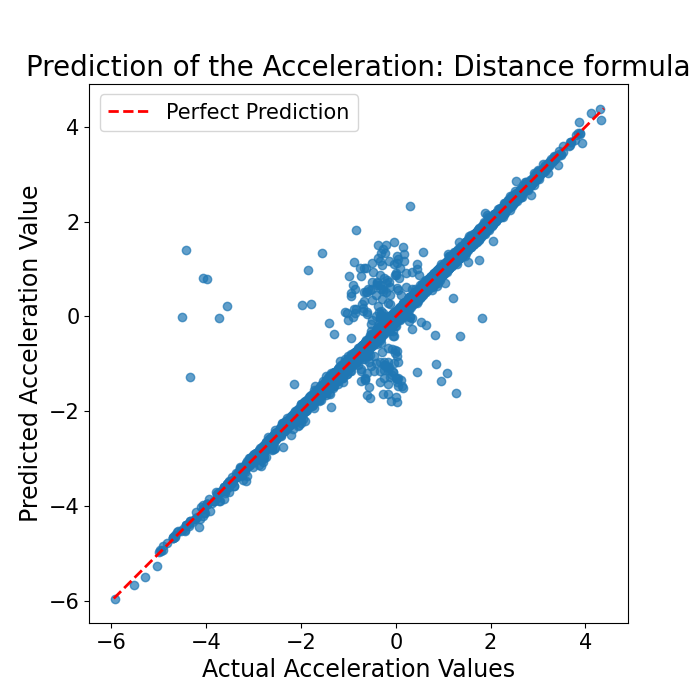
\includegraphics[width=\textwidth]{figures/graphs/Prediction of the Acceleration: Distance formula.png}
  }
    \end{minipage}
    \begin{minipage}[b]{0.49\linewidth}
      \centering
  \onslide<2>{
        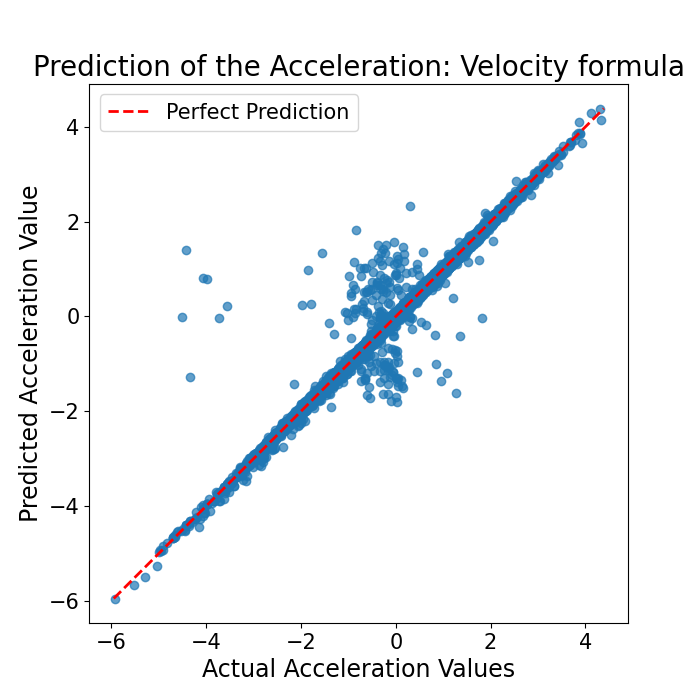
\includegraphics[width=\textwidth]{figures/graphs/Prediction of the Acceleration: Velocity formula.png}
  }
    \end{minipage}
  \end{figure}
\end{frame}

\begin{frame}
  \frametitle{Results: Comparison to the old acceleration model}

  \begin{figure}

    \centering
    \begin{minipage}[b]{0.49\linewidth}

  \onslide<1, 2>{
        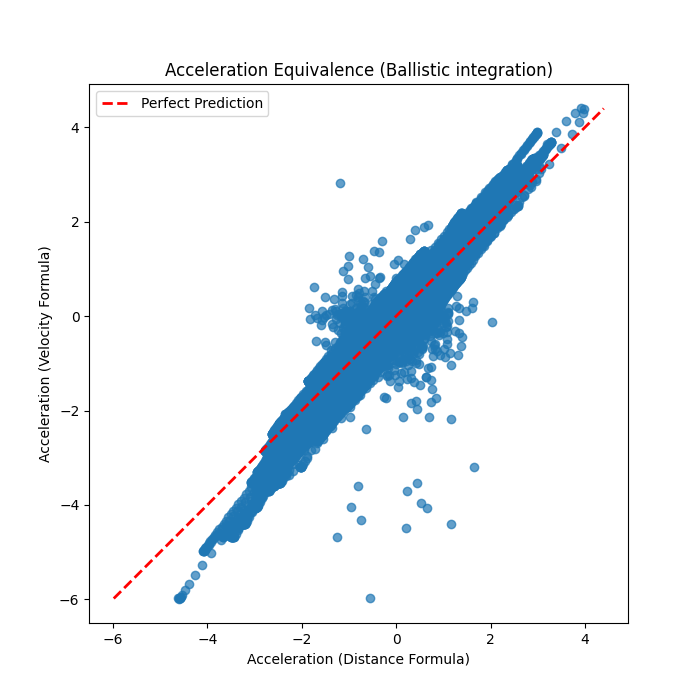
\includegraphics[width=\textwidth]{figures/graphs/Acceleration Equivalence (Ballistic integration).png}

        \centering \footnotesize MSE: 3.0786e+02
  }
    \end{minipage}
    \begin{minipage}[b]{0.49\linewidth}

  \onslide<2>{
        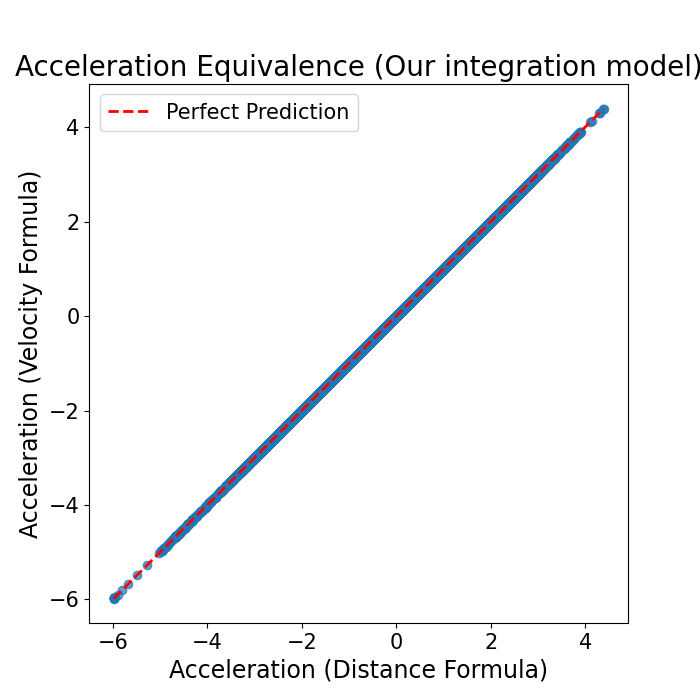
\includegraphics[width=\textwidth]{figures/graphs/Acceleration Equivalence (Our integration model).png}
        \centering \footnotesize MSE: 1.9220e-09
  }
    \end{minipage}
  \end{figure}
\end{frame}






\begin{frame}
  \frametitle{Results: Integration Method}
    Rearranging the formula to the distance and velocity gives us these results:
    \center \textit{Video demo of predicted car}
\end{frame}


\begin{frame}
  \frametitle{Results}
    Summary:
    \begin{itemize}[<+->]
      \item Successfully implemented the filtering mechanism
      \item Able to filter out X different scenarios in Y datasets
      \item Found a better integration method where the accelerations match
      \item Able to visualize the integration method and modulate the movement of a car
    \end{itemize}
\end{frame}

